\documentclass[12pt,b5paper]{ltjsarticle}

%\usepackage[margin=15truemm, top=5truemm, bottom=5truemm]{geometry}
%\usepackage[margin=10truemm,left=15truemm]{geometry}
\usepackage[margin=10truemm]{geometry}

\usepackage{amsmath,amssymb}
%\pagestyle{headings}
\pagestyle{empty}

%\usepackage{listings,url}
%\renewcommand{\theenumi}{(\arabic{enumi})}

\usepackage{graphicx}

%\usepackage{tikz}
%\usetikzlibrary {arrows.meta}
%\usepackage{wrapfig}
%\usepackage{bm}

% ルビを振る
%\usepackage{luatexja-ruby}	% required for `\ruby'

%% 核Ker 像Im Hom を定義
%\newcommand{\Img}{\mathop{\mathrm{Im}}\nolimits}
%\newcommand{\Ker}{\mathop{\mathrm{Ker}}\nolimits}
%\newcommand{\Hom}{\mathop{\mathrm{Hom}}\nolimits}

%\DeclareMathOperator{\Rot}{rot}
%\DeclareMathOperator{\Div}{div}
%\DeclareMathOperator{\Grad}{grad}
%\DeclareMathOperator{\arcsinh}{arcsinh}
%\DeclareMathOperator{\arccosh}{arccosh}
%\DeclareMathOperator{\arctanh}{arctanh}

\usepackage{url}

%\usepackage{listings}
%
%\lstset{
%%プログラム言語(複数の言語に対応,C,C++も可)
%  language = Python,
%%  language = Lisp,
%%  language = C,
%  %背景色と透過度
%  %backgroundcolor={\color[gray]{.90}},
%  %枠外に行った時の自動改行
%  breaklines = true,
%  %自動改行後のインデント量(デフォルトでは20[pt])
%  breakindent = 10pt,
%  %標準の書体
%%  basicstyle = \ttfamily\scriptsize,
%  basicstyle = \ttfamily,
%  %コメントの書体
%%  commentstyle = {\itshape \color[cmyk]{1,0.4,1,0}},
%  %関数名等の色の設定
%  classoffset = 0,
%  %キーワード(int, ifなど)の書体
%%  keywordstyle = {\bfseries \color[cmyk]{0,1,0,0}},
%  %表示する文字の書体
%  %stringstyle = {\ttfamily \color[rgb]{0,0,1}},
%  %枠 "t"は上に線を記載, "T"は上に二重線を記載
%  %他オプション:leftline,topline,bottomline,lines,single,shadowbox
%  frame = TBrl,
%  %frameまでの間隔(行番号とプログラムの間)
%  framesep = 5pt,
%  %行番号の位置
%  numbers = left,
%  %行番号の間隔
%  stepnumber = 1,
%  %行番号の書体
%%  numberstyle = \tiny,
%  %タブの大きさ
%  tabsize = 4,
%  %キャプションの場所("tb"ならば上下両方に記載)
%  captionpos = t
%}

%\usepackage{cancel}
%\usepackage{bussproofs}
%\usepackage{proof}

\begin{document}

\hrulefill

関数$f(x) = \lvert x \rvert \sin^{-1}{x}$が
点$x=0$で
微分可能かどうか調べよ。

\dotfill

関数$f(x)$が$x=a$で微分可能であるとは、
$x=a$の左側極限と右側極限が一致するときをいい、
この極限値を$x=a$における$f(x)$の微分係数という。
\begin{equation}
 f^{\prime}(a)
  =\lim _{x \rightarrow a-0} \frac{f(x)-f(a)}{x-a}
  =\lim _{x \rightarrow a+0} \frac{f(x)-f(a)}{x-a}
\end{equation}

\dotfill

$f(x)$は
$x$の値により
次のように
絶対値を外すことが出来る。
\begin{equation}
 f(x)=
  \begin{cases}
   x \sin^{-1}{x} & (x>0)\\
   0 & (x=0)\\
   -x \sin^{-1}{x} & (x<0)
  \end{cases}
\end{equation}

$x=0$における右側極限を考える。
\begin{equation}
 \lim _{x \rightarrow 0+0} \frac{f(x)-f(0)}{x-0}
  =\lim _{x \rightarrow 0+0} \frac{x\sin^{-1}{x}}{x}
  =\lim _{x \rightarrow 0+0} \sin^{-1}{x}
  =0
\end{equation}

同様に左側極限を考える。
\begin{equation}
 \lim _{x \rightarrow 0-0} \frac{f(x)-f(0)}{x-0}
  =\lim _{x \rightarrow 0-0} \frac{-x\sin^{-1}{x}}{x}
  =\lim _{x \rightarrow 0-0} \left( -\sin^{-1}{x} \right)
  =0
\end{equation}

以上により
$f(x)$は$x=0$で微分可能であり、
$f^{\prime}(0)=0$である。



\hrulefill

$y=x e^{x}$の
$I=\mathbb{R}$における
増加・減少を調べよ。

\dotfill

$y$の導関数は次の式となる。
\begin{equation}
 y^{\prime} = (x+1)e^{x}
  ,\quad
  y^{\prime\prime} = (x+2)e^{x}
\end{equation}

$y^{\prime}=0$となるのは
$x=-1$のときのみで、
$y^{\prime\prime}=0$となるのは
$x=-2$のときのみである。

%$\mathbb{R}$において
%$e^{x}>0$であり、
%$e^{x}\to\infty \; (x\to\infty)$
%と
%$e^{x}\to 0 \; (x\to-\infty)$
%となる。

$y\to\infty \; (x\to\infty)$より
$x\to\infty$のとき、
$y^{\prime}\to \infty ,\; y^{\prime\prime}\to \infty$であり、
$y\to0 \; (x\to-\infty)$より
$x\to -\infty$のとき、
$y^{\prime}\to 0 ,\; y^{\prime\prime}\to 0$
である。

\begin{center}
\begin{tabular}{|c||c|c|c|c|c|c|c|c|c|}
 \hline
 $x$ & $-\infty$ & $\cdots$ & $-2$ & $\cdots$ & $-1$ & $\cdots$ & $0$ & $\cdots$ & $\infty$ \\
 \hline
 \hline
 $y^{\prime}$ & $0$ & \multicolumn{3}{|c|}{$-$} & $0$ & \multicolumn{3}{|c|}{$+$} & $\infty$\\
 \hline
 $y^{\prime\prime}$ & $0$ & $-$ & $0$ & \multicolumn{5}{|c|}{$+$} & $\infty$ \\
 \hline
 $y$ & $0$ & & $-2 e^{-2}$ & & $-e^{-1}$ & & $0$ & & $\infty$ \\
 \hline
\end{tabular}
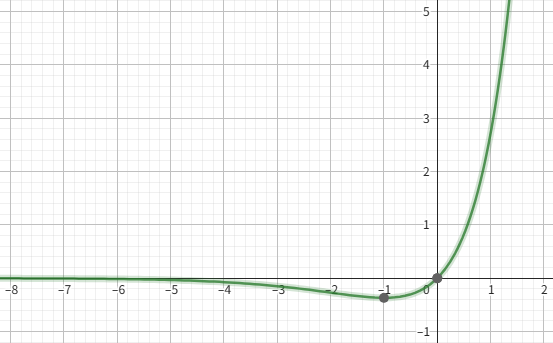
\includegraphics[scale=0.5]{xe^x.png}
\end{center}





\hrulefill

\end{document}
